\documentclass[aspectratio=169,11pt]{beamer}

\usetheme{Singapore}
\usepackage[utf8]{inputenc}
\usepackage{amsmath}
\usepackage{amsfonts}
\usepackage{amssymb}
\usepackage{graphicx}
\usepackage{hyperref}
\usepackage{booktabs}
\usepackage{listings}
\usepackage{xcolor}

% Define the settings for codechunks
\definecolor{codegreen}{rgb}{0,0.6,0}
\definecolor{codegray}{rgb}{0.5,0.5,0.5}
\definecolor{codepurple}{rgb}{0.58,0,0.82}
\definecolor{backcolour}{rgb}{0.9,0.9,0.9}
\lstdefinestyle{mystyle}{
    backgroundcolor=\color{backcolour},   
    commentstyle=\color{codegreen},
    keywordstyle=\color{magenta},
    numberstyle=\tiny\color{codegray},
    stringstyle=\color{codepurple},
    basicstyle=\ttfamily\footnotesize,
    breakatwhitespace=false,         
    breaklines=true,                 
    captionpos=b,                    
    keepspaces=true,                 
    numbers=left,                    
    numbersep=5pt,                  
    showspaces=false,                
    showstringspaces=false,
    showtabs=false,                  
    tabsize=2
}
\lstset{style=mystyle}

% Setup the bibliography
\usepackage[style=authortitle,backend=bibtex]{biblatex}
\addbibresource{bibliography.bib}
\setbeamertemplate{bibliography item}[text]
\setbeamerfont{footnote}{size=\tiny}

% Allow footnotes with no number
\newcommand\blfootnote[1]{%
  \begingroup
  \renewcommand\thefootnote{}\footnote{#1}%
  \addtocounter{footnote}{-1}%
  \endgroup
}

% Allow section title slides
\AtBeginSection[]{
  \begin{frame}
  \vfill
  \centering
  \begin{beamercolorbox}[sep=8pt,center,shadow=true,rounded=true]{title}
    \usebeamerfont{title}\insertsectionhead\par%
  \end{beamercolorbox}
  \vfill
  \end{frame}
}

\author{Dr Stephen Pederson}
\title{Lecture 7: Statistics For RNA-Seq}
\subtitle{BIOINF3005/7160: Transcriptomics Applications}
%\setbeamercovered{transparent} 
\setbeamertemplate{navigation symbols}{} 
\logo{
	
\includegraphics[scale=0.3]{figures/UoA_logo_col_vert.png} 
} 
\institute{Bioinformatics Hub, \\The University of Adelaide} 
\date{May 4th, 2020} 
\subject{BIOINF3005/7160: Transcriptomics Applications} 


\begin{document}

\begin{frame}
\titlepage
\end{frame}

\begin{frame}
\footnotesize
\tableofcontents
\end{frame}

\section{Recap of Continuous Data}

%\subsection{T-tests}

\begin{frame}{Continuous Variables}

	\begin{itemize}
		\item Continuous variables can take any value on the number line
		\begin{itemize}
			\item i.e $-\infty < x < \infty$
		\end{itemize}		 
		\item Are unbound at either limit
		\item For analysis, being continuous within the complete range of possible values is enough
		\item Microarray fluouresence intensities are bound at both extrema:
		\begin{itemize}
			\item $PM \geq 0 $ and $PM \leq 2^{16}$
		\end{itemize}
	\end{itemize}

\end{frame}

\begin{frame}{Normally Distributed Data}

	\begin{itemize}
		\item Normally distributed data \textbf{must} be continuous
		\begin{itemize}
			\item If not, the bell-curve becomes discrete
			\item Boundary points can also be problematic, but Truncated-Normal distributions exist.		
		\end{itemize}
		\item T-tests rely on the assumption of Normality
		\item Linear Regression also relies on the assumption of Normality
	\end{itemize}

\end{frame}

\subsection{Linear Regression}

\begin{frame}{Linear Regression}

	\begin{itemize}
		\item Our recent pracs have all been fitting linear regression models
		\item We attempt to fit a line through our response ($y$) and predictor ($x$) variables
		\item The interpretation is always:
	\end{itemize}
	\begin{center}
	\textbf{For a 1 unit increase in predictor $x$, we expect to see `$\ldots$' change in our response variable $y$}
	\end{center}
	
\end{frame}

\begin{frame}{Linear Regression}
	
	\begin{itemize}
		\item Our model coefficients provide this estimate of change
		\item Represent the slope of the line
		\item \textit{Predictor variables} can be discrete but \textit{response variables} must be continuous
		\begin{itemize}
			\item e.g. sample groups are a common discrete predictor
		\end{itemize}
	\end{itemize}
	
\end{frame}

\begin{frame}{Linear Regression}

For observations $\mathbf{y} = (y_1, y_2, \ldots, y_n)$ and predictors $\mathbf{x} = (x_1, x_2, \ldots, x_n)$

	\begin{align*}
	y_{i} = \beta_0 + \beta_1 x_i + \varepsilon_i
	\end{align*}

	\begin{itemize}
		\item We are trying to fit a straight line with intercept ($\beta_0$) and slope ($\beta_1$)
		\item Points never line up exactly on the line, so we need an error term $\varepsilon$
		\item The error term (also called \textit{residuals}) is $\varepsilon_i \sim \mathcal{N} (0, \sigma)$
	\end{itemize}

\end{frame}


\begin{frame}{Linear Regression}

	\begin{center}
		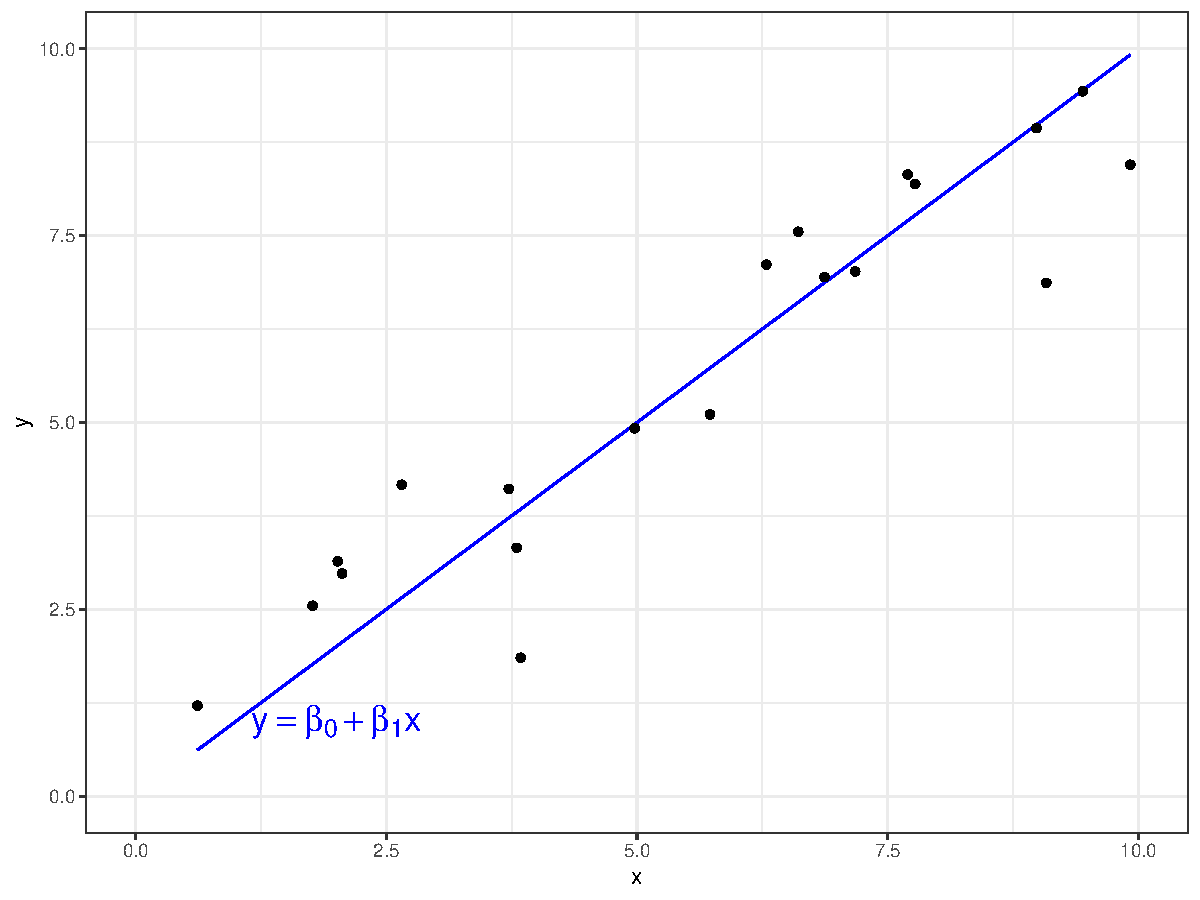
\includegraphics[scale=0.35]{figures/regPoints.pdf} 
	\end{center}

\end{frame}

\begin{frame}{Linear Regression}

	\begin{center}
		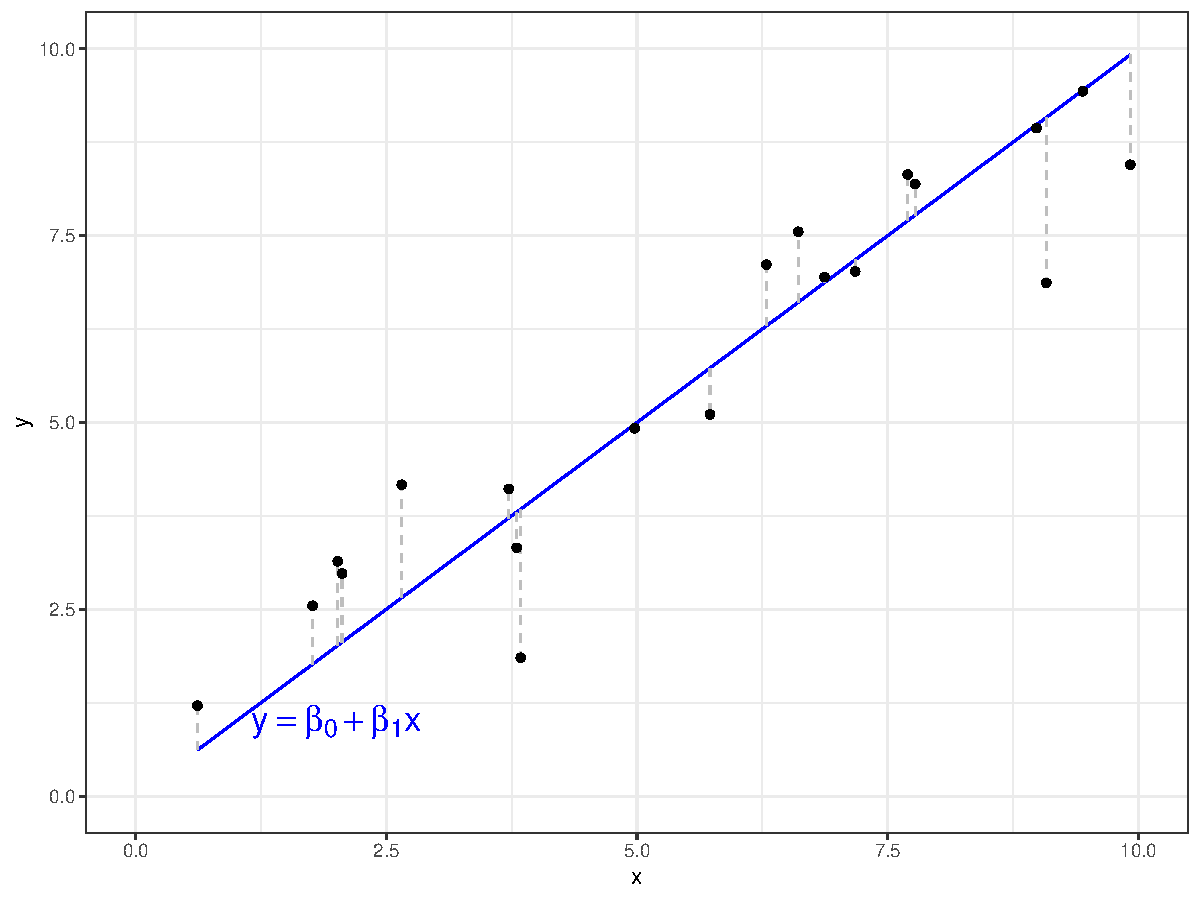
\includegraphics[scale=0.35]{figures/regPoints_resid.pdf} 
	\end{center}
	
\end{frame}

\begin{frame}{Linear Regression}

	The four assumptions of linear regression
	
	\begin{enumerate}
		\item Normality: Residuals are normally distributed
		\item Homoscedasticity: Variance is constant across the range of the data
		\item Linearity: Data is linear
		\item Observations are independent
	\end{enumerate}
	
\end{frame}

\begin{frame}{Linear Regression}

	All of these relate to the residuals: $\varepsilon_i \sim \mathcal{N}(0, \sigma)$
	
	\begin{enumerate}
		\item Normality: $\mathcal{N}$
		\item Homoscedasticity: $\sigma$
		\item Linearity: $\mu = 0$
		\item Observations are independent: (We just assume, unless we know better)
	\end{enumerate}
	

\end{frame}

\begin{frame}{Linear Regression}

	\begin{center}
		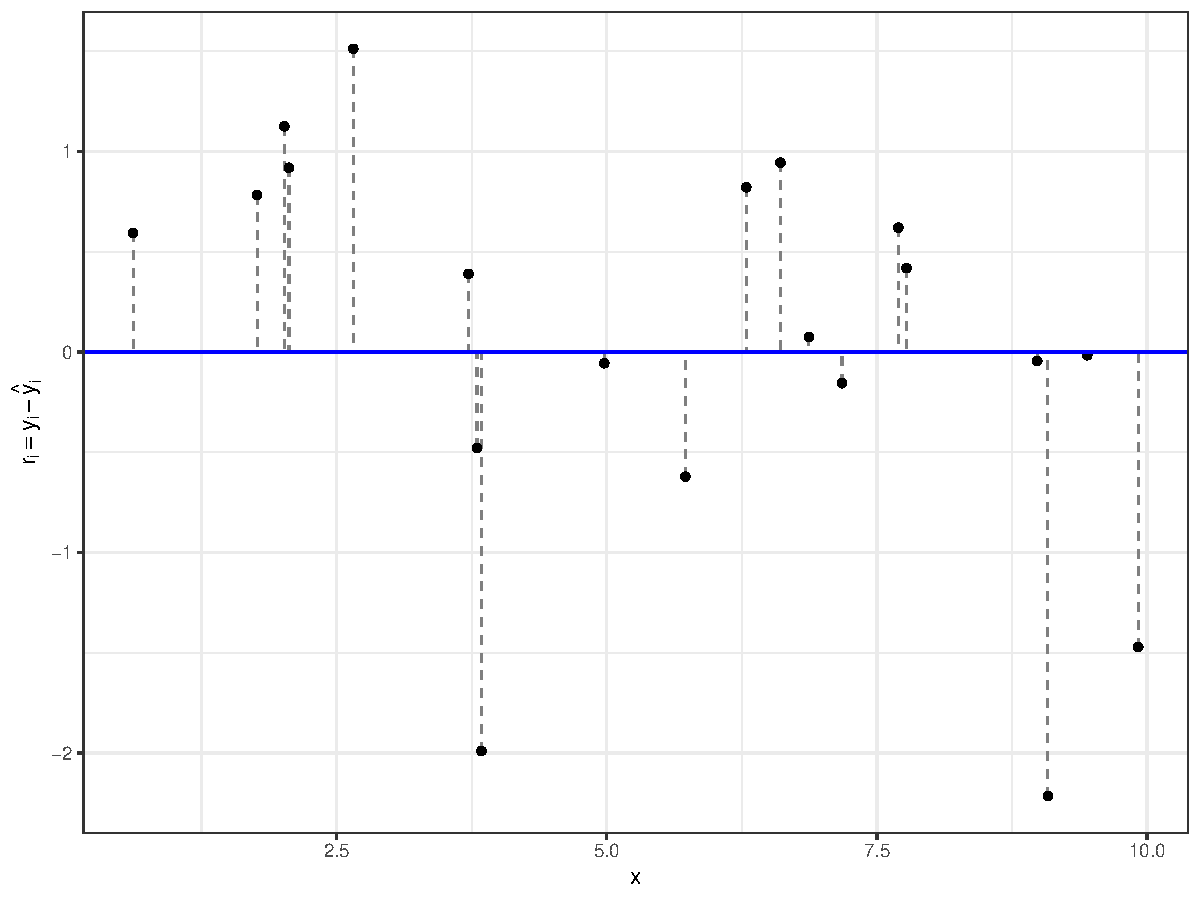
\includegraphics[scale=0.35]{figures/resid.pdf} 
	\end{center}
	
\end{frame}

\begin{frame}{Linear Regression}

	\begin{itemize}
		\item To fit a linear regression model we use least squares
	\end{itemize}
	\begin{align*}
	\hat{\beta} = ( \mathbf{X}^T \mathbf{X} )^{-1} \mathbf{X}^T\mathbf{y}
	\end{align*}
	\begin{itemize}
		\item Then we check residuals for all assumptions (linearity, normality, constant variance)
	\end{itemize}
	
\end{frame}

\begin{frame}{Microarrays}

	\begin{itemize}
		\item All of the above works well for microarrays
		\item Boundary points of 0 \& $2^{16}$ are ignored
		\item We know variance is connected to the fluorescence intensity
		\item Using $y = \log_2\hat{S}$ gives almost constant variance
		\begin{itemize}
			\item Become important when genes are DE
		\end{itemize}
		\item We can't check assumptions for every gene, but generally they hold
	\end{itemize}

\end{frame}

\begin{frame}{Microarrays}

	\begin{center}
	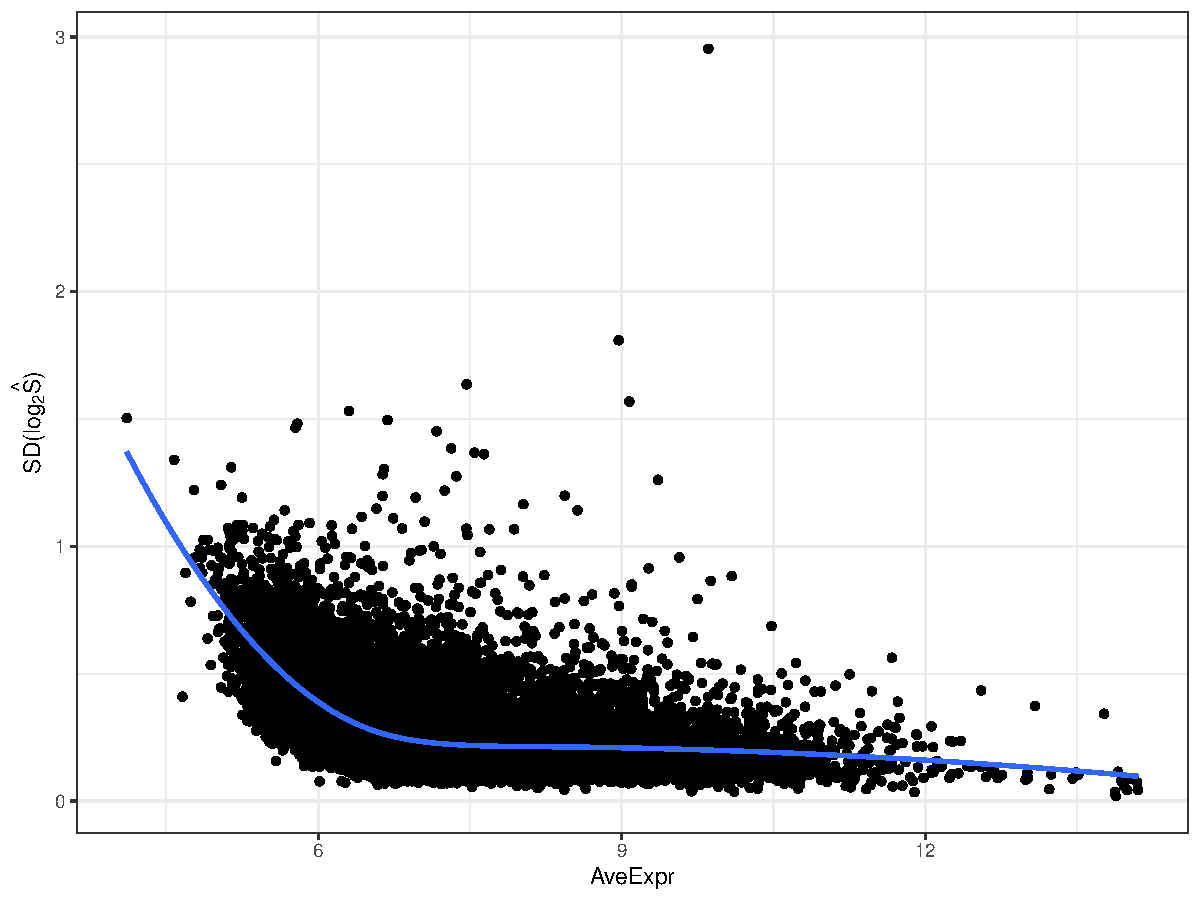
\includegraphics[scale=0.35]{figures/AvSD.pdf} 
	\end{center}

\end{frame}

\section{Discrete Distributions}

\begin{frame}{Discrete Data}

	\begin{itemize}
		\item Discrete data involves different types of measurements than continuous
		\item Common types of counts:
		\begin{enumerate}%[label=(\alph*)]
			\item Number of successes in a binary test e.g. number of 6's rolled
			\item Number of events in a fixed unit of measurement, e.g. cars passing per minute
		\end{enumerate}
		\pause
		\item The number of successes (1) can be modelled using the \textit{Binomial} and \textit{Hypergeometric} distributions
		\item The number of events (2) can be modelled using the \textit{Poisson} and \textit{Negative-Binomial} distributions
	\end{itemize}

\end{frame}

\begin{frame}{Binomial Data}

	\begin{itemize}
		\item If we have a bag of 100 balls: 20 red and 80 blue
		\item The probability of success (i.e grabbing a red ball) is $\pi = 0.2$
		\item This is the classic binomial scenario
		\item If we return the ball we've just taken $\implies \pi = 0.2$.
		\item What if we keep the ball and don't replace it?
	\end{itemize}

\end{frame}


\begin{frame}{Hypergeometric Data}

	\begin{itemize}
		\item The Hypergeometric Distribution is what happens when we sample \textbf{without replacement}
		\item The most common representation of this is a $2\times2$ table
		\item The most appropriate test is Fisher's Exact Test
	\end{itemize}

\end{frame}

\begin{frame}{Fisher's Exact Test}

	\begin{itemize}
		\item Developed by RA Fisher (prior to arrival at Adelaide)
		\item $H_0$: \textit{No association between variables} Vs $H_A$: \textit{Some association between variables}
	\end{itemize}
	\pause
	\begin{center}
		\begin{tabular}{l|rr|r}
			& \textbf{DE} & \textbf{not DE} & $n$ \\
			\toprule
			On Chr1 & 100 & 900 & 1000\\
			\textbf{Not} on Chr1 & 1000 & 19000 & 20000 \\
			\bottomrule
		\end{tabular}	
	\end{center}
	
	Here 1 in 11 DE genes is on Chr1, whilst 1 in $\sim$22 \textit{not DE} genes are on Chr1

\end{frame}

\begin{frame}{Fisher's Exact Test}

	\begin{itemize}
		\item Was there an association? ($p = 3.74\times10^{-10}$)
		\item The test is two-sided: i.e. association can be in either direction
		\item Note that once we've sampled a gene, it can't be replaced $\implies$ \textit{hypergeometric}
		\pause
		\item We use this for enrichment testing (next week) and a variation is used for Differential Expression in RNA Seq
		\item Notice there is no provision for replicates within groups under this layout
	\end{itemize}

\end{frame}

\begin{frame}{Poisson Distributed Data}

	\begin{itemize}
		\item \textit{Poisson} distributed data is based on a rate of occurrence, e.g. mobile phone networks
		\item We have a count \textit{per fixed unit} $\implies$ a rate is involved
		\item The rate parameter ($\lambda$) is the average number of number of events / unit
		\item \textbf{The standard deviation is the same as the rate}
		\item This is fundamentally different to the Normal Distribution $\implies \mu$ and $\sigma$ are independent
	\end{itemize}
	
\end{frame}

\begin{frame}[fragile]{Poisson Distributed Data}
	
	\begin{lstlisting}[language=R]
	rpois(n = 1000, lambda = 1)
	#   0   1   2   3   4   5 
	# 390 328 202  57  20   3 
	\end{lstlisting}

\end{frame}

\begin{frame}{Poisson Regression}

	\begin{itemize}
		\item To fit Poisson-distributed data, we use \textit{Generalised Linear Models} (GLM)
		\item Poisson GLMs are sometimes known as \textit{log-linear} models
		\item The formula looks the same in R, but is fitted using \textbf{Maximum Likelihood} not Least Squares
		\item The response value is fitted on the (natural) log-scale 
		\item Errors are no longer normally distributed (should be Poisson)
		\item \texttt{glm(y} $\sim$ \texttt{predictors, family = "poisson")}
	\end{itemize}

\end{frame}

\begin{frame}{Poisson Regression}

	\begin{itemize}
		\item The default formula relies in the fixed unit being identical
		\item What if we're counting trees for multiple species across multiple forests
		\item The forest size always changes \& the species distribution changes within each forest
		\item We can supply an offset term to the model which accounts for this
		\begin{itemize}
			\item Effectively standardises the unit of measurement
		\end{itemize}
	\end{itemize}

\end{frame}

\begin{frame}{Negative Binomial Data}

	\begin{itemize}
		\item What happens when our `real-world' data is more variable?
		\begin{itemize}
			\item When variance is clearly $>\lambda$
		\end{itemize}
		\item This is known as over-dispersed data
		\item Best fit using a Negative Binomial model as a GLM
		\item Essentially the same as a Poisson but with more wiggle room
	\end{itemize}

\end{frame}


\section{Applications to RNA Seq}

\subsection{Normalisation}

\begin{frame}{RNA Seq Libraries}
	\begin{itemize}
		\item After aligning to a reference and counting reads for each gene $\implies$ gene-level counts
		\item We face many familiar issues:
		\begin{itemize}
			\item How do we normalise the data?
			\item How do we test for Differential Expression?
		\end{itemize}
		\item We generally refer to each set of counts as a `library'
		\item Library Sizes are a big issue in RNA Seq
	\end{itemize}

\end{frame}

\begin{frame}{Normalisation}

	\begin{itemize}
		\item How do we adjust for library size differences
		\item Some libraries amplify well/poorly?
		\item How does this affect library composition?
		\item Do some highly expressed genes `dominate' a library?
		\item Was there a different response to GC content across individual libraries?
		\item Longer genes will also receive more counts
	\end{itemize}
	~\\
	Unlike microarrays, \textit{we don't adjust our counts directly}!

\end{frame}

\begin{frame}{Normalisation}

	\begin{itemize}
		\item Essentially we're fitting the rate of observing counts in each library
		\item This is impacted by total library size
		\item RNA-Seq data tends to be analysed using Negative Binomial Models
		\begin{itemize}
			\item Data is over-dispersed (i.e. more variable) than a Poisson model
		\end{itemize}
		\item We can use the \textit{offset} trick we introduced earlier
	\end{itemize}

\end{frame}


\begin{frame}{Normalisation}

	\begin{itemize}
		\item A naive approach would be to adjust for library sizes\\[2mm]
		\item The most common strategy is Trimmed Mean of M-values (TMM)
		\begin{itemize}
			\item Effectively adjusts for distortions in library composition and total size\\[2mm]
		\end{itemize}
		\item Can also use Conditional-Quantile Normlisation (CQN)
		\begin{itemize}
			\item This adjusts for sample-specific GC effects and/or sample-specific length effects
		\end{itemize}
	\end{itemize}

\end{frame}

\begin{frame}{TMM Normalisation}

	\begin{itemize}
		\item Here we use our $M$ and $A$ values again
		\item Assumes that most genes are not differentially expressed
		\item For a pair of samples ($k=1,2$) and a given gene $g$ with counts $y_{gk}$
	\end{itemize}
	\begin{align*}
		M_g &= \log_2 \frac{y_{g1} / N_1}{y_{g2} / N_2}\\[2mm]
		A_g &= \frac{1}{2} \left(\frac{y_{g1}}{N_1} + \frac{y_{g2}}{N_2} \right)
	\end{align*}
	\begin{itemize}
		\item In all of the above $N_k$ represents the total library size
	\end{itemize}

\end{frame}

\begin{frame}{TMM Normalisation}

	\begin{itemize}
		\item Data across all genes is trimmed 30\% ($M$-values) and 5\% ($A$-values)
		\item The sum of the weighted trimmed $M$-values is then calculated
		\item A \textit{sample-level} normalisation factor is calculated by comparing to a reference sample
		\item This value is provided to the model as an offset
	\end{itemize}

\end{frame}

\begin{frame}{CQ Normalisation}

	\begin{itemize}
		\item GC content and gene length doesn't change across samples
		\item Sometimes libraries respond differently during library preparation
		\item May be PCR-related or fragmentation-related
		\item CQN provides an \textit{gene-level} and \textit{sample-level} offset
	\end{itemize}

\end{frame}

\subsection{Differential Expression}

\begin{frame}{Dispersions}

	\begin{itemize}
		\item Under the NB model there is Poisson variability ($\mu$) + overdispersion ($\varphi$)
		\item $E(Y) = \mu$ and Var$(Y) = \mu + \varphi\mu^2$, with $\varphi > 0$
		\item This is estimated as an overall value, and a gene-level value
		\item Specifically designed to handle unequal library sizes
		\begin{itemize}
			\item $\hat{\varphi}$ is estimated using a quantile Conditional Maximum Likelihood model (qCML)\footfullcite{SmythExactTest}
			\item The qCML procedure requires calculation of pseudo-counts, or pseudo-data
		\end{itemize}
	\end{itemize}

\end{frame}

\begin{frame}{The Exact Test}

	\begin{itemize}
		\item For a simple 2 group comparison, an Exact Test can be used
		\item By using the qCML estimates, pseudo-data is identically distributed across samples
		\item Can be pooled within groups for Fisher's Exact Test\footfullcite{SmythExactTest}
		\item Provides a $p$-value for Differential Expression
		\begin{itemize}
			\item $H_0: \lambda_1 = \lambda_2$ with $H_A: \lambda_1 \neq \lambda_2$
			\item logFC is effectively the $\Delta\lambda$ on the $\log_2$ scale
		\end{itemize}
	\end{itemize}

\end{frame}

\begin{frame}{GLM Approaches}

	\begin{itemize}
		\item For more general approaches a GLM approach can be taken using a Negative Binomial as the underlying distribution
		\item Can fit simple 2-group comparisons or more complex designs
		\item Under these approaches, trended dispersions are used
		\item Analogous to moderated variances for the moderated T-test
		\begin{itemize}
			\item A different Empirical Bayes model is used
			\item Reduces false positives and false negatives simultaneously
		\end{itemize}
	\end{itemize}

\end{frame}

\begin{frame}{GLM Approaches}

	\begin{itemize}
		\item The effect of any predictor on the counts can be modelled
		\item The latest approach is to use the Quasi-Likelihood GLM fit (\texttt{glmQLFit()})
		\item This has been shown to be the most reliable model
		\begin{itemize}
			\item The original GLM models in \texttt{edgeR} don't strictly control the FDR\footfullcite{pmid23104842}
		\end{itemize}
	\end{itemize}

\end{frame}

\begin{frame}{Differential Expression Testing}

	\begin{itemize}
		\item For Microarray data, we perform a T-test on each model coefficient
		\item This is not possible under GLM approaches
		\item Instead we perform Likelihood Ratio Tests
		\begin{itemize}
			\item Tests the `Goodness of Fit' of two models
			\item One with the model term, the other without
		\end{itemize}
		\item For QL-GLM we can use a Quasi-Likelihood F-test
		\item Analogous to an ANOVA test
	\end{itemize}

\end{frame}

\begin{frame}{voom}

	\begin{itemize}
		\item An alternative to all of the above might be to transform the counts into continuous data
		\item How would we handle the mean-variance relationship?
		\item The voom approach is based on using Counts/Million, or logCPM\footfullcite{pmid24485249}
	\end{itemize}

\end{frame}


\begin{frame}{voom}
	
	\begin{center}
	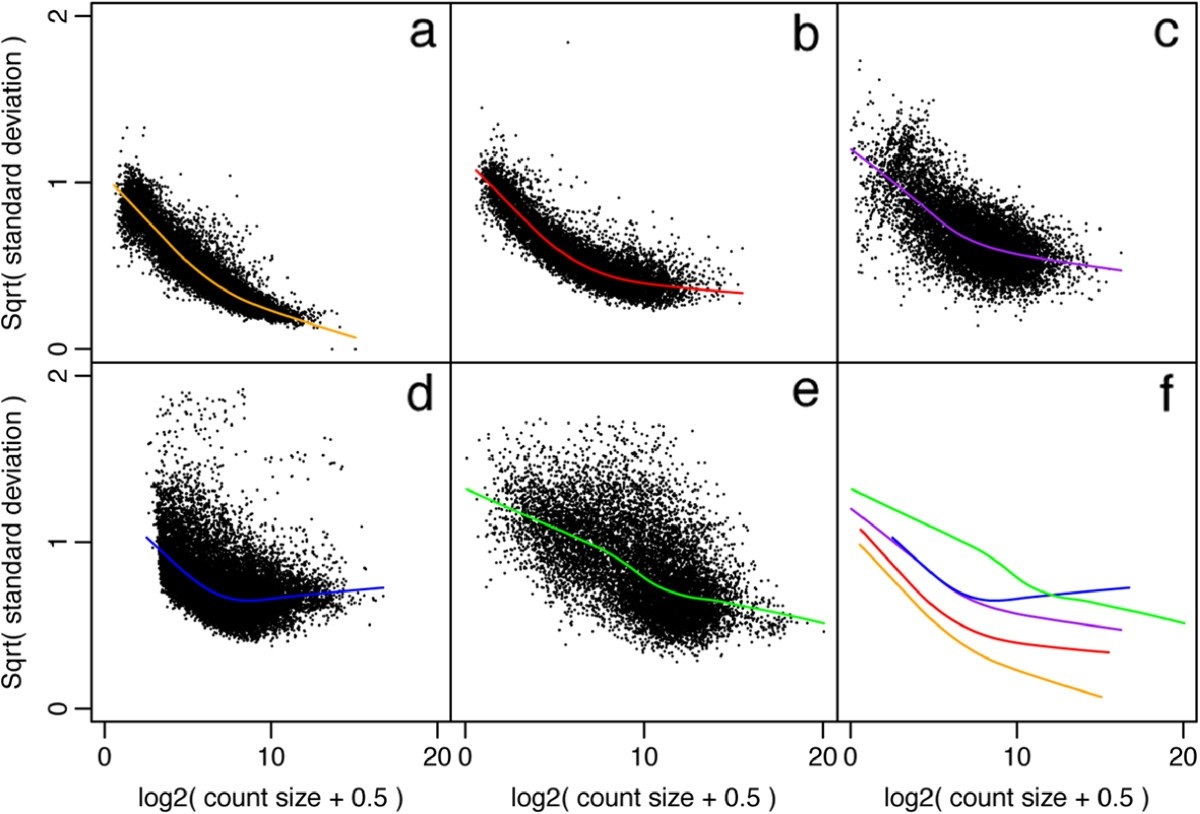
\includegraphics[scale=0.2]{figures/cpm_mean_var.jpg} 
	\end{center}

\end{frame}


\begin{frame}{voom}

	
	\begin{center}
	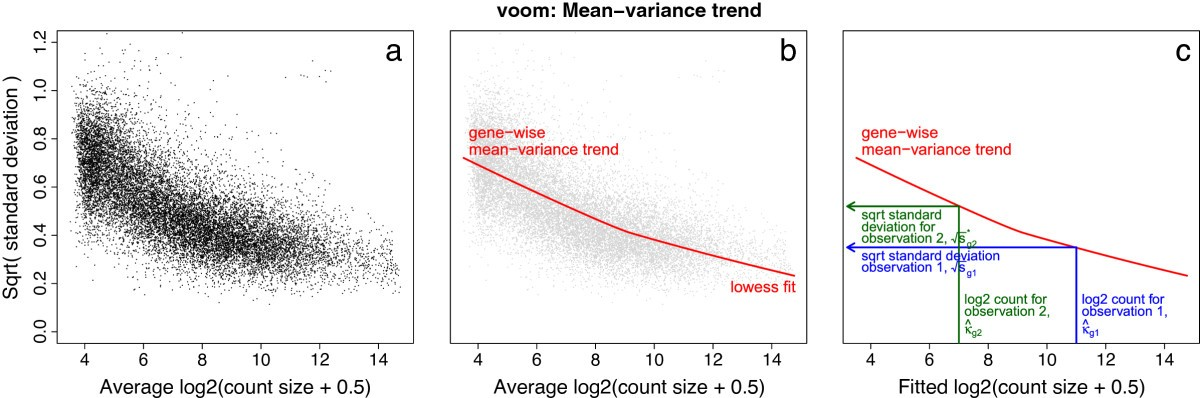
\includegraphics[scale=0.25]{figures/voom.jpg} 
	\end{center}

	\begin{itemize}
		\item Predicted counts are obtained by fitting the CPM values
		\item Using the lowess curve based on counts, predicted standard deviations are obtained
		\item The inverse of predicted standard deviations (but squared) are the weights
		\item We can fit using limma and all assumptions of normality are back on the table
	\end{itemize}

\end{frame}

\begin{frame}{Why Normality?}

	\begin{itemize}
		\item The suite of statistical tools available for Normal data is vary broad
		\item Weighted regression, Mixed-effects/Nested Models, T-tests
		\item Voom brings this back into play
	\end{itemize}

\end{frame}

\begin{frame}{A Final Word}

	\begin{itemize}
		\item A common measure for gene expression is Counts / Million (CPM) or logCPM
		\item Very intuitive measure and useful for visualisation
		\item Only voom uses them for fitting data, by managing the mean-variance relationship
		\item Nearly all other models use the raw counts for fitting
		\begin{itemize}
			\item Early approaches used RPKM and FPKM $\implies$ now discredited
			\item Another common value is Transcripts Per Kilobase Million (TPM) $\implies$ incorporates gene length
		\end{itemize}
		\item CPM is good across samples; TPM is good within samples
	\end{itemize}
	
\end{frame}

\end{document}
